\chapter{Multivariate models}\label{chap7}

We describe how to perform Bayesian inference in multivariate response models, including multivariate regression, seemingly unrelated regression, instrumental variables, and the multivariate probit model. In particular, we present the posterior distributions of the parameters and demonstrate several applications and simulations. Additionally, we show how to perform inference in these models using three levels of programming skills: GUI, packages, and programming the algorithms from scratch. Finally, we provide some mathematical and computational exercises.

Remember that we can run our GUI typing

\begin{tcolorbox}[enhanced,width=4.67in,center upper,
	fontupper=\large\bfseries,drop shadow southwest,sharp corners]
	\textit{R code. How to display our graphical user interface}
	\begin{VF}
		\begin{lstlisting}[language=R]
	shiny::runGitHub("besmarter/BSTApp", launch.browser = T)
\end{lstlisting}
	\end{VF}
\end{tcolorbox} 

in the \textbf{R} package console or any \textbf{R} code editor. However, users should see Chapter \ref{chapGUI} for seeing other options.

\section{Multivariate regression}\label{sec71}

A complete presentation of this model is given in Section \ref{sec44}. We show here the setting, and the posterior distributions for facility in exposition. In particular, there are $M$ multiply dependent variables which share the same set of regressors, and their stochastic errors are contemporaneously correlated. In particular, $\bm{Y}=\left[{\bm{y_{1}}} \ {\bm{y_{2}}} \ \ldots \ {\bm{y_{M}}}\right]$ is a $ N\times M$ matrix that is generated by $\bm{Y}=\bm{X}\bm{B}+\bm{U}$ where $\bm{X}$ is an $ N\times K$ matrix of regressors, $\bm{B}=\left[\bm{\beta}_{1} \ \bm{\beta}_{2} \ldots \bm{\beta}_{M}\right]$ is a $ K\times M$ matrix of parameters, and $\bm{U}=\left[\bm{\mu}_{1} \ \bm{\mu}_{2}\ldots \bm{\mu}_{M}\right]$ is a matrix of stochastic random errors such that $\bm{\mu}_i\sim{N}(\bm{0},\bm{\Sigma})$, $i=1,2,\dots,N$ is each row of $\bm{U}$.

The prior is given by $\bm{B}\mid\bm{\Sigma}\sim{N}(\bm{B}_0,\bm{V}_0, \bm{\Sigma})$ and $\bm{\Sigma}\sim{I}{W}(\bm{\Psi}_0,\alpha_0)$. Therefore, the conditional posterior distributions are
\begin{equation*}
	\bm{B}\mid\bm{\Sigma}, \bm{Y}, \bm{X} \sim{N}(\bm{B}_n, \bm{V}_n, \bm{\Sigma}), 
\end{equation*}
\begin{equation*}
	\bm{\Sigma}\mid \bm{Y}, \bm{X} \sim {I}{W}(\bm{\Psi}_n, \alpha_n),
\end{equation*}

where $\bm{V}_n=(\bm{X}^{\top}\bm{X}+\bm{V}_0^{-1})^{-1}$, $\bm{B}_n=\bm{V}_n(\bm{V}_0^{-1}\bm{B}_0 + \bm{X}^{\top}\bm{X}\hat{\bm{B}})$, $\hat{\bm{B}}=(\bm{X}^{\top}\bm{X})^{-1}\bm{X}^{\top}\bm{Y}$, ${\bm{S}}=(\bm{Y}-\bm{X}\hat{\bm{B}})^{\top}(\bm{Y}-\bm{X}\hat{\bm{B}})$, $\bm{\Psi}_n = {\bm{\Psi}}_{0}+{\bm{S}}+{\bm{B}}_{0}^{\top}{\bm{V}}_{0}^{-1}{\bm{B}}_{0}+\widehat{\bm{B}}^{\top}{\bm{X}}^{\top}{\bm{X}}\widehat{\bm{B}}-{\bm{B}}_n^{\top}{\bm{V}}_n^{-1}{\bm{B}}_n$, and $\alpha_n = \alpha_0 + N$. We can use a Gibbs sampling algorithm in this model since the conditional posterior distributions are standard.\\

\textbf{Example: The effect of institutions on per capita gross domestic product}

To illustrate multivariate regression models, we use the dataset provided by \cite{Acemoglu2001}, who analyzed the effect of property rights on economic growth.

We begin with the following \textit{simultaneous structural} economic model:\footnote{This model captures the potential underlying economic relationship between the variables.}
\begin{align}\label{eq:str1}
	\log(\text{pcGDP95}_i) &= \beta_1 + \beta_2 \text{PAER}_i + \beta_3 \text{Africa} + \beta_4 \text{Asia} + \beta_5 \text{Other} + u_{1i},
\end{align}
\begin{align}\label{eq:str2}
	\text{PAER}_i &= \alpha_1 + \alpha_2 \log(\text{pcGDP95}_i) + \alpha_3 \log(\text{Mort}_i) + u_{2i},
\end{align}
where \textit{pcGDP95}, \textit{PAER}, and \textit{Mort} represent the per capita gross domestic product (GDP) in 1995, the average index of protection against expropriation between 1985 and 1995, and the settler mortality rate during the period of colonization, respectively. \textit{Africa}, \textit{Asia}, and \textit{Other} are indicator variables for continents, with \textit{America} serving as the baseline group.

In this model, there is \textit{simultaneous causality} due to the contemporaneous effect of \textit{GDP} on \textit{PAER}, and vice versa. Therefore, estimating Equations \ref{eq:str1} and \ref{eq:str2} without accounting for this phenomenon results in posterior mean estimates that are \textit{biased} and \textit{inconsistent} from a sampling (frequentist) perspective.\footnote{Note that $\mathbb{E}[u_1\text{PAER}]\neq 0$, which means failing to meet a necessary condition for obtaining \textit{unbiased} and \textit{consistent} estimators of $\bm{\beta}$. See Exercise 1.} A potential strategy to address this issue is to estimate the \textit{reduced-form} model, i.e., a model without \textit{simultaneous causality}, where all \textit{endogenous variables} are functions of \textit{exogenous variables}. The former are determined within the model (e.g., $\log(\text{pcGDP95}_i)$ and \textit{PAER} in this example), while the latter are determined outside the model (e.g., $\log(\text{Mort}_i)$, \textit{Africa}, \textit{Asia}, and \textit{Other} in this example).

Replacing Equation \ref{eq:str2} into Equation \ref{eq:str1}, and solving for $\log(\textit{pcGDP95})$,
\begin{align}\label{eq:red1}
	\log(\text{pcGDP95}_i)=\pi_1+\pi_2\log(\text{Mort}_i)+\pi_3 \text{Africa}+\pi_4 \text{Asia}+\pi_5 \text{Other}+e_{1i}.   
\end{align}
Then, by substituting Equation \ref{eq:red1} into Equation \ref{eq:str2}, and solving for \textit{PAER}, we obtain
\begin{align}\label{eq:red2}
	\text{PAER}_i = \gamma_1 + \gamma_2 \log(\text{Mort}_i) + \gamma_3 \text{Africa} + \gamma_4 \text{Asia} + \gamma_5 \text{Other} + e_{2i},
\end{align}
where $\pi_2 = \frac{\beta_2\alpha_3}{1 - \beta_2\alpha_2}$ and $\gamma_2 = \frac{\alpha_3}{1 - \beta_2\alpha_2}$, given that $\beta_2 \alpha_2 \neq 1$, i.e., independent equations (see Exercise 2).

Observe that Equations \ref{eq:red1} and \ref{eq:red2} have the form of a multivariate regression model, where the common set of regressors is $\bm{X} = \left[\log(\text{Mort}) \ \text{Africa} \ \text{Asia} \ \text{Other}\right]$ and the common set of dependent variables is $\bm{Y} = \left[\log(\text{pcGDP95}) \ \text{PAER}\right]$. Therefore, we can estimate this model using the setup outlined in this section.

In the first stage, we estimate the parameters of the \textit{reduced-form} model (Equations \ref{eq:red1} and \ref{eq:red2}), but the main interest lies in estimating the parameters of the \textit{structural} model (Equations \ref{eq:str1} and \ref{eq:str2}). A valid question is whether we can recover (identify) the \textit{structural} parameters from the \textit{reduced-form} parameters. There are two criteria to answer this question: the order condition, which is necessary, and the rank condition, which is both necessary and sufficient.\footnote{We should clarify that the posterior distribution of the structural parameters, $\pi(\boldsymbol{\beta},\boldsymbol{\alpha}\mid \boldsymbol{\gamma},\boldsymbol{\pi},\mathbf{Y},\mathbf{X})$, is proportional to the prior distribution of the structural parameters conditional on the reduced-form parameters, $\pi(\boldsymbol{\beta},\boldsymbol{\alpha}\mid \boldsymbol{\gamma},\boldsymbol{\pi})$.	In other words, it is only the prior distribution of the reduced-form parameters that is updated by the sample information. The updating of the structural parameters occurs solely through the reduced-form parameters. See Section~9.3 in \cite{zellner1996introduction} for details.}\\
 
\textbf{The order condition}

Given a system of equations with $M$ endogenous variables and $K$ exogenous variables (including the intercept), there are two ways to assess the order condition:
\begin{itemize}
	\item The parameters of an equation in the system are identified if there are at least $M-1$ variables excluded from that equation (\textit{exclusion restrictions}). The equation is \textit{exactly identified} if the number of excluded variables equals $M-1$, and \textit{over-identified} if the number of excluded variables is greater than $M-1$.
	\item The parameters of equation $m$ in the system are identified if $K-K_m \geq M_m-1$, where $K_m$ and $M_m$ are the number of exogenous and endogenous variables in equation $m$, respectively. The $m$-th equation is \textit{exactly identified} if $K-K_m = M_m-1$, and \textit{over-identified} if $K-K_m > M_m-1$.
\end{itemize}

Otherwise, the structural parameters are \textit{under-identified}.

We can see from Equations \ref{eq:str1} and \ref{eq:str2} in this example that $K=5$, $M=2$, $K_1=4$, $K_2=2$, $M_1=2$ and $M_2=2$. This means that $K-K_1=1=M-1$ and $K-K_2=3>M-1=1$, that is, the order condition says that both equations satisfy the necessary condition of identification, the first equation would be \textit{exactly identified}, and the second equation would be \textit{over identified}. Observe that there is one excluded variable from the first equation, and there are three excluded variables from the second equation.\\

\textbf{The rank condition}

The rank condition (necessary and sufficient) states that, given a \textit{structural} model with $M$ equations (and $M$ endogenous variables), an equation is identified if and only if there exists at least one nonzero determinant of an $(M-1)\times(M-1)$ matrix constructed from the variables excluded from the equation under analysis but included in at least one other equation of the system. Otherwise, the structural parameters are said to be \textit{under-identified}.


It is useful to build the \textit{identification matrix} to implement the \textit{rank} condition. Table \ref{tab:71} shows this matrix in this example.

\begin{table}[!h]
	%\noautomaticrules
	\tabletitle{Identification matrix.}\label{tab:71}%
	\begin{tabular}{ccccccc}
		$\log(\text{pcGDP95})$ & PAER & Constant & $\log(\text{Mort})$ & Africa & Asia & Other \\
		\hline
		1 & -$\beta_2$ & -$\beta_1$ & 0 & -$\beta_3$ & -$\beta_4$ & -$\beta_5$\\
		-$\alpha_2$ & 1 & $-\alpha_1$ & -$\alpha_3$ & 0 & 0 & 0 \\
	\end{tabular}
\end{table}

The only excluded variable in the $\log(\text{pcGDP95})$ equation is $\log(\text{Mort})$. Therefore, there is only one matrix that can be constructed using the excluded variables from this equation, which is $[-\alpha_3]$ (see column 4 in Table \ref{tab:71}). The determinant of this matrix is $-\alpha_3$, and as long as this coefficient is nonzero (i.e., $\alpha_3 \neq 0$), meaning that the mortality rate is relevant in the PAER equation, the coefficients in the $\log(\text{pcGDP95})$ equation are \textit{exactly identified}. For example, $\beta_2 = \frac{\pi_2}{\gamma_2}$, which represents the effect of property rights on GDP, is exactly identified.

It is crucial to observe the importance of excluding $\log(\text{Mort})$ from the $\log(\text{pcGDP95})$ equation, while including $\log(\text{Mort})$ in the PAER equation. This is known as the \textit{exclusion restriction}, which requires the presence of an exogenous source of variability in the PAER equation to help identify the $\log(\text{pcGDP95})$ equation. The presence of relevant exogenous sources of variability is an essential factor in the identification, estimation, and inference of \textit{structural} parameters.

As for the identification of the \textit{structural} parameters in the PAER equation, there are three potential matrices that can be constructed: $[-\beta_3]$, $[-\beta_4]$, and $[-\beta_5]$ (see columns 5, 6, and 7 in Table \ref{tab:71}). As long as any of these parameters are relevant in the $\log(\text{pcGDP95})$ equation, the PAER equation is identified. In this case, the PAER equation is \textit{over-identified}, meaning there are multiple ways to estimate the parameters in this equation. For example, $\alpha_2 = \gamma_3/\pi_3 = \gamma_4/\pi_4 = \gamma_5/\pi_5$ (see Exercise 2).

In general, recovering the \textit{structural} parameters from the \textit{reduced-form} parameters can be challenging due to the need for relevant identification restrictions, which can be difficult to find in some applications.\footnote{Good introductory-level textbooks on identification in linear systems include \cite[Chap. ~19]{gujarati2009basic} and \cite[Chap. ~16]{wooldridge2016introductory}.}

For this example, we set non-informative priors: $\bm{B}_0 = \left[\bm{0}_5 \ \bm{0}_5\right]$, $\bm{V}_0 = 100 \bm{I}_K$, $\bm{\Psi}_0 = 5 \bm{I}_2$, and $\alpha_0 = 5$.\footnote{Note that we are setting the priors in the \textit{reduced-form} model. This may have unintended consequences for the posterior distributions of the \textit{structural} parameters, which are ultimately the parameters of interest to researchers. For further discussion, see \cite[p.~302]{koop2003bayesian}.} Once our GUI is displayed (see the beginning of this chapter), we should follow Algorithm \ref{alg:MultReg} to run multivariate linear models in the GUI (see Chapter \ref{chapGUI} for details, particularly on how to set the data set).
\begin{algorithm}[h!]
	\caption{Multivariate linear model}\label{alg:MultReg}
	\begin{algorithmic}[1]  		 			
		\State Select \textit{Multivariate Models} on the top panel
		\State Select \textit{Simple Multivariate} model using the left radio button
		\State Upload the dataset selecting first if there is header in the file, and the kind of separator in the \textit{csv} file of the dataset (comma, semicolon, or tab). Then, use the \textit{Browse} button under the \textbf{Choose File} legend
		\State Select MCMC iterations, burn-in and thinning parameters using the \textit{Range sliders}
		\State Select the number of dependent variables in the box \textbf{Number of endogenous variables: m}
		\State Select the number of independent variables (including the intercept) in the box \textbf{Number of exogenous variables: k}
		\State Set the hyperparameters: mean vectors, covariance matrix, degrees of freedom, and the scale matrix. This step is not necessary as by default our GUI uses non-informative priors
		\State Click the \textit{Go!} button
		\State Analyze results
		\State Download posterior chains and diagnostic plots using the \textit{Download Posterior Chains} and \textit{Download Posterior Graphs} buttons
	\end{algorithmic} 
\end{algorithm}

The following \textbf{R} code shows how to perform the Gibss sampling algorithm in this example using the dataset \textit{4Institutions.csv}. We ask to run this example using the \textit{rmultireg} command from the \textit{bayesm} package as an exercise. We find that the posterior mean \textit{structural} effect of property rights on GDP is 0.98, and the 95\% credible interval is (0.56, 2.87). This means that there is evidence supporting a positive effect of property rights on gross domestic product. 

\begin{tcolorbox}[enhanced,width=4.67in,center upper,
	fontupper=\large\bfseries,drop shadow southwest,sharp corners]
	\textit{R code. The effect of institutions on per capita GDP}
	\begin{VF}
		\begin{lstlisting}[language=R]
rm(list = ls())
set.seed(12345)
DataInst <- read.csv("https://raw.githubusercontent.com/besmarter/BSTApp/refs/heads/master/DataApp/4Institutions.csv", sep = ",", header = TRUE, quote = "")
attach(DataInst)
Y <- cbind(logpcGDP95, PAER)
X <- cbind(1, logMort, Africa, Asia, Other)
M <- dim(Y)[2]
K <- dim(X)[2]
N <- dim(Y)[1]
# Hyperparameters
B0 <- matrix(0, K, M)
c0 <- 100
V0 <- c0*diag(K)
Psi0 <- 5*diag(M)
a0 <- 5
# Posterior parameters
Bhat <- solve(t(X)%*%X)%*%t(X)%*%Y 
S <- t(Y - X%*%Bhat)%*%(Y - X%*%Bhat)
Vn <- solve(solve(V0) + t(X)%*%X) 
Bn <- Vn%*%(solve(V0)%*%B0 + t(X)%*%X%*%Bhat)
Psin <- Psi0 + S + t(B0)%*%solve(V0)%*%B0 + t(Bhat)%*%t(X)%*%X%*%Bhat - t(Bn)%*%solve(Vn)%*%Bn
an <- a0 + N
#Posterior draws
s <- 10000 #Number of posterior draws
SIGs <- replicate(s, LaplacesDemon::rinvwishart(an, Psin))
BsCond <- sapply(1:s, function(s) {MixMatrix::rmatrixnorm(n = 1, mean=Bn, U = Vn,V = SIGs[,,s])})
summary(coda::mcmc(t(BsCond)))
SIGMs <- t(sapply(1:s, function(l) {gdata::lowerTriangle(SIGs[,,l], diag=TRUE, byrow=FALSE)}))
summary(coda::mcmc(SIGMs))
hdiBs <- HDInterval::hdi(t(BsCond), credMass = 0.95) # Highest posterior density credible interval
hdiBs
hdiSIG <- HDInterval::hdi(SIGMs, credMass = 0.95) # Highest posterior density credible interval
hdiSIG
beta2 <- BsCond[2,]/BsCond[7,] 
summary(coda::mcmc(beta2)) # Effect of property rights on GDP
Iterations = 1:10000
Thinning interval = 1 
Number of chains = 1 
Sample size per chain = 10000 
1. Empirical mean and standard deviation for each variable,
plus standard error of the mean:
Mean             SD       Naive SE Time-series SE 
0.9796        16.8430         0.1684         0.1684 
2. Quantiles for each variable:
2.5%    25%    50%    75%  97.5% 
0.5604 0.7984 0.9677 1.2329 2.8709 
\end{lstlisting}
	\end{VF}
\end{tcolorbox} 

\section{Seemingly unrelated regression}\label{sec72}

In seemingly unrelated regression (SUR) models, there are $M$ dependent variables, each with potentially different regressors, such that the stochastic errors are contemporaneously correlated. The model is given by:
\[
\bm{y}_m = \bm{X}_m \bm{\beta}_m + \bm{\mu}_m,
\]
where $\bm{y}_m$ is an $N$-dimensional vector of observations, $\bm{X}_m$ is an $N \times K_m$ matrix of regressors, $\bm{\beta}_m$ is a $K_m$-dimensional vector of location parameters, and $\bm{\mu}_m$ is an $N$-dimensional vector of stochastic errors, for $m = 1, 2, \dots, M$.

Let $\bm{\mu}_i = \left[\mu_{i1} \ \mu_{i2} \ \dots \ \mu_{iM}\right]^{\top}$, where $\bm{\mu}_i \sim {N}(\bm{0}, \bm{\Sigma})$. Stacking the $M$ equations, we can write the model as:
\[
\bm{y} = \bm{X} \bm{\beta} + \bm{\mu},
\]
where $\bm{y} = \left[\bm{y}_1^{\top} \ \bm{y}_2^{\top} \ \dots \ \bm{y}_M^{\top}\right]^{\top}$ is an $MN$-dimensional vector, $\bm{\beta} = \left[\bm{\beta}_1^{\top} \ \bm{\beta}_2^{\top} \ \dots \ \bm{\beta}_M^{\top}\right]^{\top}$ is a $K$-dimensional vector with $K = \sum_{m=1}^M K_m$, and $\bm{X}$ is an $MN \times K$ block-diagonal matrix composed of the individual $\bm{X}_m$, i.e.,
\[
\bm{X} = \begin{bmatrix}
	\bm{X}_1 & \bm{0} & \dots & \bm{0} \\
	\bm{0} & \bm{X}_2 & \dots & \bm{0} \\
	\vdots & \vdots & \ddots & \vdots \\
	\bm{0} & \bm{0} & \dots & \bm{X}_M
\end{bmatrix}.
\]
Similarly, the vector of errors is given by $\bm{\mu} = \left[\bm{\mu}_1^{\top} \ \bm{\mu}_2^{\top} \ \dots \ \bm{\mu}_M^{\top}\right]^{\top}$, which is an $MN$-dimensional vector of stochastic errors, with $\bm{\mu} \sim {N}(\bm{0}, \bm{\Sigma} \otimes \bm{I}_N)$.

The likelihood function for the parameters is then:
\[
p(\bm{\beta}, \bm{\Sigma} \mid \bm{y}, \bm{X}) \propto |\bm{\Sigma}|^{-N/2} \exp\left\{ -\frac{1}{2} (\bm{y} - \bm{X} \bm{\beta})^{\top} (\bm{\Sigma}^{-1} \otimes \bm{I}_N) (\bm{y} - \bm{X} \bm{\beta}) \right\}.
\]

Using independent priors $\pi(\bm{\beta})\sim{N}(\bm{\beta}_0,\bm{B}_0)$ and $\pi(\bm{\Sigma}^{-1})\sim{W}(\alpha_0,\bm{\Psi}_0)$, the posterior distributions are
\begin{equation*}
	\bm{\beta}\mid\bm{\Sigma}, \bm{y}, \bm{X} \sim {N}(\bm{\beta}_n, \bm{B}_n), 
\end{equation*}
\begin{equation*}
	\bm{\Sigma}^{-1}\mid\bm{\beta}, \bm{y}, \bm{X} \sim {W}(\alpha_n, \bm{\Psi}_n),
\end{equation*}

where $\bm{B}_n=(\bm{X}^{\top}(\bm{\Sigma}^{-1}\otimes \bm{I}_N )\bm{X}+\bm{B}_0^{-1})^{-1}$, $\bm{\beta}_n=\bm{B}_n(\bm{B}_0^{-1}\bm{\beta}_0 + \bm{X}^{\top}(\bm{\Sigma}^{-1}\otimes \bm{I}_N)\bm{y})$, $\alpha_n = \alpha_0 + N$ and $\bm{\Psi}_n = (\bm{\Psi}_0^{-1} + \bm{U}^{\top}\bm{U})^{-1}$, where $\bm{U}$ is an $N\times M$ matrix whose columns are $\bm{y}_m-\bm{X}_m\bm{\beta}_m$. 

We can demonstrate, through straightforward yet tedious algebra, that by defining $\bm{y}_i = [y_{i1} \ y_{i2} \ \dots \ y_{iM}]$ and
\begin{align*}
	\bm{X}_i=\begin{bmatrix}
		x_{1i}^{\top} & \bm{0} & \dots & \bm{0}\\
		\bm{0} & x_{2i}^{\top} & \dots & \bm{0}\\
		\vdots & \vdots & \ddots & \vdots\\
		\bm{0} & \bm{0} & \dots & x_{Mi}^{\top}\\
	\end{bmatrix},
\end{align*} 
we alternatively have $\bm{B}_n=(\bm{B}_0^{-1}+\sum_{i=1}^N \bm{X}_i^{\top}\bm{\Sigma}^{-1}\bm{X}_i)^{-1}$, $\bm{\beta}_n=\bm{B}_n(\bm{B}_0^{-1}\bm{\beta}_0+\sum_{i=1}^N \bm{X}_i^{\top}\bm{\Sigma}^{-1}\bm{y}_i)$ and $\bm{\Psi}_n = (\bm{\Psi}_0^{-1} + \sum_{i=1}^N (\bm{y}_i-\bm{X}_i^{\top}\bm{\beta}) (\bm{y}_i-\bm{X}_i^{\top}\bm{\beta})^{\top})^{-1}$.

Observe that we have standard conditional posteriors, thus, we can employ a Gibbs sampling algorithm to get the posterior draws.\\

\textbf{Example: Utility demand}

Let's use the dataset \textit{Utilities.csv} to estimate a seemingly unrelated regression (SUR) model for utilities. We adopt the same setting as in Exercise 14 of Chapter \ref{chap4}, where we estimate a multivariate regression model while omitting households with no consumption in any utility. In this exercise, we observe that not all regressors are relevant for the demand of electricity, water, and gas. Thus, we estimate the following model:
\begin{align*}
	\log(\text{electricity}_i) & = \beta_1 + \beta_2\log(\text{electricity price}_i)+\beta_3\log(\text{water price}_i)\\
	&+\beta_4\log(\text{gas price}_i)+\beta_5\text{IndSocio1}_i+\beta_6\text{IndSocio2}_i+\beta_7\text{Altitude}_i\\
	&+\beta_8\text{Nrooms}_i+\beta_9\text{HouseholdMem}_i+\beta_{10}\log(\text{Income}_i)+\mu_{i1}\\
	\log(\text{water}_i) & = \alpha_1 + \alpha_2\log(\text{electricity price}_i)+\alpha_3\log(\text{water price}_i)\\
	&+\alpha_4\log(\text{gas price}_i)+\alpha_5\text{IndSocio1}_i+\alpha_6\text{IndSocio2}_i\\
	&+\alpha_7\text{Nrooms}_i+\alpha_8\text{HouseholdMem}_i+\mu_{i2}\\
	\log(\text{gas}_i) & = \gamma_1 + \gamma_2\log(\text{electricity price}_i)+\gamma_3\log(\text{water price}_i)\\
	&+\gamma_4\log(\text{gas price}_i)+\gamma_5\text{IndSocio1}_i+\gamma_6\text{IndSocio2}_i+\gamma_7\text{Altitude}_i\\
	&+\gamma_8\text{Nrooms}_i+\gamma_9\text{HouseholdMem}_i+\mu_{i3},
\end{align*} 
where electricity, water, and gas represent the monthly consumption of electricity (kWh), water (m$^3$), and gas (m$^3$) of Colombian households. The dataset includes information on 2,103 households, with details on the average prices of electricity (USD/kWh), water (USD/m$^3$), and gas (USD/m$^3$), as well as indicators of the socioeconomic conditions of the neighborhood where the household is located (IndSocio1 being the lowest and IndSocio3 the highest). Additionally, there is information on whether the household is located in a municipality situated at over 1,000 meters above sea level, the number of rooms in the house, the number of household members, and monthly income (USD).

Since each equation has a different set of regressors, and we suspect correlation between the stochastic errors of the three equations, we should estimate a seemingly unrelated regression (SUR) model. We expect unobserved correlation across these equations because we are modeling utilities, and in some cases, a single provider handles all three services and issues one bill.

Algorithm \ref{alg:SUR} demonstrates how to estimate SUR models using our GUI. Our GUI utilizes the command \textit{rsurGibbs} from the \textit{bayesm} package in \textbf{R} software. See Chapter \ref{chapGUI} for further details, including instructions on how to set up the dataset, and check the templates available in our GitHub repository (\textbf{https://github.com/besmarter/BSTApp}) in the \textbf{DataApp} and \textbf{DataSim} folders.

The following code shows how to program this application using this package. We use 10000 MCMC iterations, $\bm{\beta}_0=\bm{0}_{27}$, $\bm{B}_0=100\bm{I}_{27}$, $\alpha_0=5$ and $\bm{\Psi}=5\bm{I}_3$.

We find that the posterior median estimates of the own-price elasticities of demand for electricity, water, and gas are -1.88, -0.36, and -0.62, respectively, and none of the 95\% credible intervals encompass 0. This means that a 1\% increase in the prices of electricity, water, and gas results in a 1.88\%, 0.36\%, and 0.62\% decrease in the monthly consumption of these utilities, respectively.\footnote{This is an example where concerns about \textit{biased} and \textit{inconsistent} posterior mean estimates may arise, for instance, due to \textit{simultaneous causality} between quantity and demand. These concerns are valid; however, we are using micro-level data, which implies no demand-supply simultaneity. Additionally, the utility providers operate in regulated natural monopoly markets, which mitigates endogeneity from searching provider strategies. Finally, we took prices directly from provider records, which avoids potential price measurement errors \cite{ramirez2024welfare}.} In general, there is evidence supporting the relevance of all regressors in these equations, with a few exceptions, and unobserved correlation in the demand for these services, which further supports the use of a SUR model in this application.

\begin{algorithm}[h!]
	\caption{Seemingly unrelated regression}\label{alg:SUR}
	\begin{algorithmic}[1]  		 			
		\State Select \textit{Multivariate Models} on the top panel
		\State Select \textit{Seemingly Unrelated Regression} model using the left radio button
		\State Upload the dataset selecting first if there is header in the file, and the kind of separator in the \textit{csv} file of the dataset (comma, semicolon, or tab). Then, use the \textit{Browse} button under the \textbf{Choose File} legend
		\State Select MCMC iterations, burn-in and thinning parameters using the \textit{Range sliders}
		\State Select the number of dependent variables in the box \textbf{Number of endogenous variables: m}
		\State Select the number of independent variables in the box \textbf{TOTAL number Exogenous Variables: k}. This is the sum of all exogenous variables over all equations including intercepts. In the example of \textbf{Utility demand}, it is equal to 27
		\State Set the hyperparameters: mean vectors, covariance matrix, degrees of freedom, and the scale matrix. This step is not necessary as by default our GUI uses non-informative priors
		\State Click the \textit{Go!} button
		\State Analyze results
		\State Download posterior chains and diagnostic plots using the \textit{Download Posterior Chains} and \textit{Download Posterior Graphs} buttons
	\end{algorithmic} 
\end{algorithm}


\begin{tcolorbox}[enhanced,width=4.67in,center upper,
	fontupper=\large\bfseries,drop shadow southwest,sharp corners]
	\textit{R code. Utility demand in Colombia}
	\begin{VF}
		\begin{lstlisting}[language=R]
rm(list = ls())
set.seed(010101)
library(dplyr)
DataUt <- read.csv("https://raw.githubusercontent.com/besmarter/BSTApp/refs/heads/master/DataApp/Utilities.csv", sep = ",", header = TRUE, quote = "")
DataUtEst <- DataUt %>%  
filter(Electricity != 0 & Water !=0 & Gas != 0)
attach(DataUtEst)
y1 <- log(Electricity); y2 <- log(Water); y3 <- log(Gas)
X1 <- cbind(1, LnPriceElect, LnPriceWater, LnPriceGas, IndSocio1, IndSocio2, Altitude, Nrooms, HouseholdMem, Lnincome)
X2 <- cbind(1, LnPriceElect, LnPriceWater, LnPriceGas, IndSocio1, IndSocio2, Nrooms, HouseholdMem)
X3 <- cbind(1, LnPriceElect, LnPriceWater, LnPriceGas, IndSocio1, IndSocio2, Altitude, Nrooms, HouseholdMem)
regdata <- NULL
regdata[[1]] <- list(y = y1, X = X1); regdata[[2]] <- list(y = y2, X = X2); regdata[[3]] <- list(y = y3, X = X3)
M <- length(regdata); K1 <- dim(X1)[2]; K2 <- dim(X2)[2]; K3 <- dim(X3)[2] 
K <- K1 + K2 + K3
# Hyperparameters
b0 <- rep(0, K); c0 <- 100; B0 <- c0*diag(K); V <- 5*diag(M); a0 <- M
Prior <- list(betabar = b0, A = solve(B0), nu = a0, V = V)
#Posterior draws
S <- 10000; keep <- 1; Mcmc <- list(R = S, keep = keep)
PosteriorDraws <- bayesm::rsurGibbs(Data = list(regdata = regdata), Mcmc = Mcmc, Prior = Prior)
\end{lstlisting}
	\end{VF}
\end{tcolorbox}

\begin{tcolorbox}[enhanced,width=4.67in,center upper,
	fontupper=\large\bfseries,drop shadow southwest,sharp corners]
	\textit{R code. Utility demand in Colombia, results}
	\begin{VF}
		\begin{lstlisting}[language=R]
Bs <- PosteriorDraws[["betadraw"]]
Names <- c("Const", "LnPriceElect", "LnPriceWater", "LnPriceGas", "IndSocio1", "IndSocio2", 
"Altitude", "Nrooms", "HouseholdMem", "Lnincome", "Const",
"LnPriceElect", "LnPriceWater", "LnPriceGas", "IndSocio1", "IndSocio2", 
"Nrooms", "HouseholdMem","Const",
"LnPriceElect", "LnPriceWater", "LnPriceGas", "IndSocio1", "IndSocio2", 
"Altitude", "Nrooms", "HouseholdMem")
colnames(Bs) <- Names
summary(coda::mcmc(Bs))
2. Quantiles for each variable:
					2.5%      25%       50%      75%    97.5%
Const         0.44452  1.03120  1.342407  1.65192  2.25376
LnPriceElect -2.39679 -2.06328 -1.882706 -1.70369 -1.36996
LnPriceWater -0.44221 -0.38678 -0.356850 -0.32669 -0.26969
LnPriceGas   -0.21655 -0.13777 -0.098191 -0.05902  0.01872
IndSocio1    -0.87630 -0.78653 -0.737701 -0.68840 -0.59675
IndSocio2    -0.24601 -0.18286 -0.151440 -0.11896 -0.05681
Altitude     -0.27080 -0.23838 -0.220742 -0.20385 -0.17259
Nrooms        0.04596  0.06178  0.070023  0.07835  0.09422
HouseholdMem  0.06600  0.07994  0.086857  0.09411  0.10785
Lnincome      0.03836  0.05421  0.062957  0.07165  0.08717
Const         0.88957  1.73496  2.169638  2.62170  3.47216
LnPriceElect -0.81956 -0.31624 -0.054075  0.21132  0.71842
LnPriceWater -0.49559 -0.40995 -0.364248 -0.32026 -0.23639
LnPriceGas    0.06075  0.16754  0.226690  0.28570  0.39476
IndSocio1    -0.64203 -0.50302 -0.427819 -0.35226 -0.21315
IndSocio2    -0.50401 -0.40949 -0.359821 -0.31063 -0.21199
Nrooms        0.05688  0.08023  0.093139  0.10555  0.12968
HouseholdMem  0.10041  0.12065  0.131506  0.14260  0.16314
Const        -2.28569 -1.58566 -1.220078 -0.84612 -0.14787
LnPriceElect -2.42484 -2.01228 -1.797269 -1.57889 -1.16396
LnPriceWater -0.10684 -0.03923 -0.004088  0.03153  0.09905
LnPriceGas   -0.76526 -0.67445 -0.625899 -0.57734 -0.48125
IndSocio1    -0.91381 -0.80243 -0.744909 -0.68577 -0.57341
IndSocio2    -0.31791 -0.24388 -0.203300 -0.16415 -0.09012
Altitude      0.24896  0.29099  0.311668  0.33256  0.37278
Nrooms        0.06050  0.07921  0.089386  0.09943  0.11793
HouseholdMem  0.14467  0.16144  0.170024  0.17843  0.19431
summary(coda::mcmc(PosteriorDraws[["Sigmadraw"]]))
2. Quantiles for each variable:
				2.5%     25%     50%     75%  97.5%
var1 0.19912 0.20822 0.21332 0.21863 0.2290
var2 0.08183 0.09284 0.09870 0.10475 0.1160
var3 0.05121 0.05973 0.06426 0.06882 0.0781
var4 0.08183 0.09284 0.09870 0.10475 0.1160
var5 0.47763 0.49934 0.51131 0.52387 0.5493
var6 0.07318 0.08653 0.09351 0.10079 0.1145
var7 0.05121 0.05973 0.06426 0.06882 0.0781
var8 0.07318 0.08653 0.09351 0.10079 0.1145
var9 0.29523 0.30900 0.31654 0.32428 0.3397
\end{lstlisting}
	\end{VF}
\end{tcolorbox}

We ask in the Exercise 5 to run this application using our GUI and the information in the dataset \textit{Utilities.csv}. Observe that this file should be modified to agree the structure that requires our GUI (see the dataset \textit{5Institutions.csv} in the folder \textit{DataApp} of our GitHub repository -\textbf{https://github.com/besmarter/BSTApp}- for a template). In addition, we ask to program from scratch the Gibbs sampler algorithm in this application.  

\section{Instrumental variable}\label{sec73}

This inferential approach is used when there are \textit{endogeneity} issues, that is, when the stochastic error is not independent of the regressors. This, in turn, generates \textit{bias} in posterior mean estimates when we use an inferential approach that does not account for this issue. \textit{Endogeneity} can be caused by \textit{simultaneous causality}, \textit{omitting relevant correlated variables}, or \textit{measurement error} in the regressors.\footnote{See \cite[Chap. ~15]{wooldridge2016introductory} for an introductory treatment of instrumental variables in the Frequentist inferential approach.}

Let’s specify the dependent variable as a linear function of one endogenous regressor and some exogenous regressors. That is, 
\[
y_{i} = \bm{x}_{ei}^{\top}\bm{\beta}_1 + \beta_s x_{si} + \mu_{i}
\]
where \(x_{si} = \bm{x}_{ei}^{\top}\bm{\gamma}_1 + \bm{z}_i^{\top}\bm{\gamma}_2 + v_{i}\), \(x_s\) is the variable that generates the endogeneity issues (\(\mathbb{E}[\mu \mid x_{s}] \neq 0\)), \(\bm{x}_e\) are \(K_1\) exogenous regressors (\(\mathbb{E}[\mu \mid \bm{x}_{e}] = \bm{0}\)), and \(\bm{z}\) are \(K_2\) instruments. The instruments are regressors that drive \(x_s\) (\(\mathbb{E}[x_{s} \bm{z}] \neq \bm{0}\)), but do not have a direct effect on \(y\) (\(\mathbb{E}[y \bm{z} \mid x_s] = \bm{0}\)). The equation for \(y\) is called the \textit{structural equation}, and it is the equation that the researcher is ultimately interested in.

Assuming $(u_{i},v_i)^{\top}\stackrel{i.i.d.} {\thicksim} {N}(0,\bm{\Sigma})$, $\bm{\Sigma}=[\sigma_{lm}]$, $l,m=1,2$, the likelihood function is
\begin{align*}
	p(\bm{\beta},\bm{\gamma},\bm{\Sigma}\mid \bm{y},\bm{X},\bm{Z})=\frac{1}{(2\pi)^\frac{N}{2}|\bm{\Sigma}|^\frac{N}{2}}\exp\left\{-\frac{1}{2}\sum_{i=1}^N(y_i-\bm{x}_i^{\top}\bm{\beta}, x_{si} -\bm{w}_i^{\top}\bm{\gamma})\bm{\Sigma}^{-1}
	\begin{pmatrix}
		y_i-\bm{x}_i^{\top}\bm{\beta} \\
		x_{si}-\bm{w}_i^{\top}\bm{\gamma}
	\end{pmatrix}
	\right\},
\end{align*}
where $\bm{\beta}=\left[\bm{\beta}_1^{\top} \ \beta_s\right]^{\top}$, $\bm{\gamma}=\left[\bm{\gamma}_1^{\top} \ \bm{\gamma}_2^{\top}\right]^{\top}$, $\bm{x}_i=\left[\bm{x}_{ei}^{\top} \ x_{si}\right]^{\top}$ and $\bm{w}_i=\left[\bm{x}_{ei}^{\top} \ \bm{z}_{i}^{\top}\right]^{\top}$.

We obtain the standard conditional posterior densities by specifying the following independent priors: 
\[
\bm{\gamma} \sim N(\bm{\gamma}_0, \bm{G}_0), \quad \bm{\beta} \sim N(\bm{\beta}_0, \bm{B}_0), \quad \bm{\Sigma}^{-1} \sim {W}(\alpha_0, \bm{\Psi}_0).
\]
In particular, the conditional distributions are:
\begin{equation*}
	\bm{\beta} \mid \bm{\gamma}, \bm{\Sigma}, \bm{y}, \bm{X}, \bm{Z} \sim N(\bm{\beta}_n, \bm{B}_n),
\end{equation*}
\begin{equation*}
	\bm{\gamma} \mid \bm{\beta}, \bm{\Sigma}, \bm{y}, \bm{X}, \bm{Z} \sim N(\bm{\gamma}_n, \bm{G}_n),
\end{equation*}
\begin{equation*}
	\bm{\Sigma}^{-1} \mid \bm{\beta}, \bm{\gamma}, \bm{y}, \bm{X}, \bm{Z} \sim {W}(\alpha_n, \bm{\Psi}_n),
\end{equation*}
where
\[
\bm{\beta}_n = \bm{B}_n \left( \bm{B}_0^{-1} \bm{\beta}_0 + \omega_1^{-1} \sum_{i=1}^{N} \left[ \bm{x}_i \left( y_i - \frac{\sigma_{12}(x_{si} - \bm{w}_i^{\top} \bm{\gamma})}{\sigma_{22}} \right) \right] \right),
\]
\[
\bm{B}_n = \left( \omega_1^{-1} \sum_{i=1}^{N} \bm{x}_i \bm{x}_i^{\top} + \bm{B}_0^{-1} \right)^{-1}, \quad \omega_1 = \sigma_{11} - \frac{\sigma_{12}^2}{\sigma_{22}},
\]
\[
\bm{G}_n = \left( \omega_2^{-1} \sum_{i=1}^{N} \bm{w}_i \bm{w}_i^{\top} + \bm{G}_0^{-1} \right)^{-1}, \quad \bm{\gamma}_n = \bm{G}_n \left( \bm{G}_0^{-1} \bm{\gamma}_0 + \omega_2^{-1} \sum_{i=1}^{N} \left[ \bm{w}_i \left( x_{si} - \frac{\sigma_{12} (y_i - \bm{x}_i^{\top} \bm{\beta})}{\sigma_{11}} \right) \right] \right),
\]
\[
\omega_2 = \sigma_{22} - \frac{\sigma_{12}^2}{\sigma_{11}}, \quad \bm{\Psi}_n = \left[ \bm{\Psi}_0^{-1} + \sum_{i=1}^N \begin{pmatrix} y_i - \bm{x}_i^{\top} \bm{\beta} \\ x_{si} - \bm{w}_i^{\top} \bm{\gamma} \end{pmatrix} (y_i - \bm{x}_i^{\top} \bm{\beta}, x_{si} - \bm{w}_i^{\top} \bm{\gamma}) \right]^{-1},
\]
\[
\alpha_n = \alpha_0 + N, \quad \sigma_{lj} \text{ are the elements of } \bm{\Sigma}.
\]

We also use a Gibbs sampling algorithm in this model since we have standard conditional posterior distributions.\\

\textbf{Example: Simulation exercise}

Let's simulate the simple process $y_i=\beta_1+\beta_2x_{si}+\mu_i$ and $x_{si}=\gamma_1+\gamma_2z_i+v_i$ where $[\mu_i \ v_i]^{\top}\sim N(\bm{0},\bm{\Sigma})$, $\bm{\Sigma}=[\sigma_{lj}]$ such that $\sigma_{12}\neq 0$, $i=1,2,\dots,100$.

Observe that $\mu\mid v\sim N\left(\frac{\sigma_{12}}{\sigma_{22}}v,\sigma_{11}-\frac{\sigma_{21}^2}{\sigma_{22}}\right)$, this implies that $\mathbb{E}[\mu\mid x_s]=\mathbb{E}[\mu\mid v]=\frac{\sigma_{12}}{\sigma_{22}}v\neq 0$ given $\sigma_{12}\neq 0$ and $\mathbb{E}[\mu\mid z]=0$.
Let's set all location parameters equal to 1, and $\sigma_{11}=\sigma_{22}=1$, $\sigma_{12}=0.8$, and $z\sim N(0,1)$. We know from the large sampling properties of the posterior mean that this converge to the maximum likelihood estimator (see Section \ref{sec11}, and \cite{Lehmann2003,van2000asymptotic}), which in this setting is $\hat{\beta}_2=\frac{\widehat{Cov}(x_s,y)}{\widehat{Var}(x_s)}$ which converges in probability to $\beta_2+\frac{\sigma_{12}}{\sigma_{22}Var(x_s)}=\beta_2+\frac{\sigma_{12}}{\sigma_{22}(\gamma_2^2Var(z)+\sigma_{22})}=1.4$, that is, the asymptotic bias when using the posterior mean of a linear regression without taking into account endogeneity is 0.4 in this example.

We assess the sampling performance of the Bayesian estimators by simulating this setting 100 times. The following code demonstrates how to do this using a linear model that does not account for the \textit{endogeneity} issue (see Section \ref{sec61}), as well as how to implement the instrumental variable model using the function \textit{rivGibbs} from the package \textit{bayesm}.\footnote{It seems that this function does not account for the effect of the exogenous regressors in the equation for the endogenous regressors.} In this setup, we use \( \bm{B}_0 = 1000 \bm{I}_2 \), \( \bm{\beta}_0 = \bm{0}_2 \), and the parameters of the inverse gamma distribution are set to 0.0005. For the instrumental variable model, we additionally set \( \bm{\gamma}_0 = \bm{0}_2 \), \( \bm{G}_0 = 1000 \bm{I}_2 \), \( \alpha_0 = 3 \), and \( \bm{\Psi}_0 = 3 \bm{I}_2 \).

\begin{tcolorbox}[enhanced,width=4.67in,center upper,
	fontupper=\large\bfseries,drop shadow southwest,sharp corners]
	\textit{R code. Simulation exercise, sampling properties ordinary and instrumental models}
	\begin{VF}
		\begin{lstlisting}[language=R]
rm(list = ls()); set.seed(010101)
N <- 100; k <- 2
B <- rep(1, k); G <- rep(1, 2); s12 <- 0.8
SIGMA <- matrix(c(1, s12, s12, 1), 2, 2)
z <- rnorm(N); Z <- cbind(1, z); w <- matrix(1,N,1); S <- 100
U <- replicate(S, MASS::mvrnorm(n = N, mu = rep(0, 2), SIGMA))
x <- G[1] + G[2]*z + U[,2,]; y <- B[1] + B[2]*x + U[,1,]
# Hyperparameters
d0 <- 0.001/2; a0 <- 0.001/2
b0 <- rep(0, k); c0 <- 1000; B0 <- c0*diag(k)
B0i <- solve(B0); g0 <- rep(0, 2)
G0 <- 1000*diag(2); G0i <- solve(G0)
nu <- 3; Psi0 <- nu*diag(2)
# MCMC parameters
mcmc <- 5000; burnin <- 1000
tot <- mcmc + burnin; thin <- 1
# Gibbs sampling
Gibbs <- function(x, y){
	Data <- list(y = y, x = x, w = w, z = Z)
	Mcmc <- list(R = mcmc, keep = thin, nprint = 0)
	Prior <- list(md = g0, Ad = G0i, mbg = b0, Abg = B0i, nu = nu, V = Psi0)
	RestIV <- bayesm::rivGibbs(Data = Data, Mcmc = Mcmc, Prior = Prior)
	PostBIV <- mean(RestIV[["betadraw"]])
	ResLM <- MCMCpack::MCMCregress(y ~ x + w - 1, b0 = b0, B0 = B0i, c0 = a0, d0 = d0)
	PostB <- mean(ResLM[,1]); Res <- c(PostB,PostBIV)
	return(Res)
}
PosteriorMeans <- sapply(1:S, function(s) {Gibbs(x = x[,s], y = y[,s])})
rowMeans(PosteriorMeans)
Model <- c(replicate(S, "Ordinary"), replicate(S, "Instrumental"))
postmeans <- c(t(PosteriorMeans))
df <- data.frame(postmeans, Model, stringsAsFactors = FALSE)
library(ggplot2); library(latex2exp)
histExo <- ggplot(df, aes(x = postmeans, fill = Model)) + geom_histogram(bins = 40, position = "identity", color = "black", alpha = 0.5) + labs(title = "Overlayed Histograms", x = "Value", y = "Count") + scale_fill_manual(values = c("blue", "red")) + geom_vline(aes(xintercept = mean(postmeans[1:S])), color = "black", linewidth = 1, linetype = "dashed") + geom_vline(aes(xintercept = mean(postmeans[101:200])), color = "black", linewidth = 1, linetype = "dashed") + geom_vline(aes(xintercept = B[2]), color = "green", linewidth = 1, linetype = "dashed") + xlab(TeX("$E[\\beta_2]$")) + ylab("Frequency") + ggtitle("Histogram: Posterior means simulating 100 samples") 
histExo 
\end{lstlisting}
	\end{VF}
\end{tcolorbox}

Figure \ref{fig71} displays the histograms of the posterior means of \( \beta_2 \) using the ordinary model, which does not account for endogeneity, and the instrumental variable model. On one hand, the mean of the posterior means for the ordinary model is 1.41 (black dashed line in the red histogram), implying a bias of 0.41, which is very close to the population bias of 0.40. On the other hand, the mean of the posterior means for the instrumental variable model is 1.04 (black dashed line in the blue histogram), which is close to the population value of \( \beta_2 = 1 \) (green dashed line).

We also observe that the histogram of the posterior means for the ordinary model is less dispersed. That is, this estimator is more efficient, which is a well-known result in the Frequentist inferential approach when comparing ordinary least squares and two-stage least squares (see \cite[Chap. ~5]{wooldridge2010econometric}).

Two very important aspects in the instrumental variables literature are the \textit{weakness} and \textit{exogeneity} of the instruments. The former refers to how strong the relationship is between the instruments and the endogenous regressors, while the latter refers to the independence of the instruments from the stochastic error in the \textit{structural equation}. In Exercise 6, we ask you to use the previous code as a baseline to study these two aspects. Observe the link between the \textit{weakness} and \textit{exogeneity} of the instrument, and the \textit{exclusion restrictions} (\( \mathbb{E}[x_s \bm{z}] \neq \bm{0} \) and \( \mathbb{E}[y \bm{z} \mid x_s] = \bm{0} \)). This is the point of departure of \cite{Conley2012}, who propose assessing the plausibility of the \textit{exclusion restrictions} by defining \textit{plausible exogeneity} as having prior information that the effect of the instrument in the \textit{structural equation} is near zero, but perhaps not exactly zero. See Chapter \ref{chap12} for more details about instrumental variables, particularly Section \ref{chap12_4}.
 
\begin{figure}
	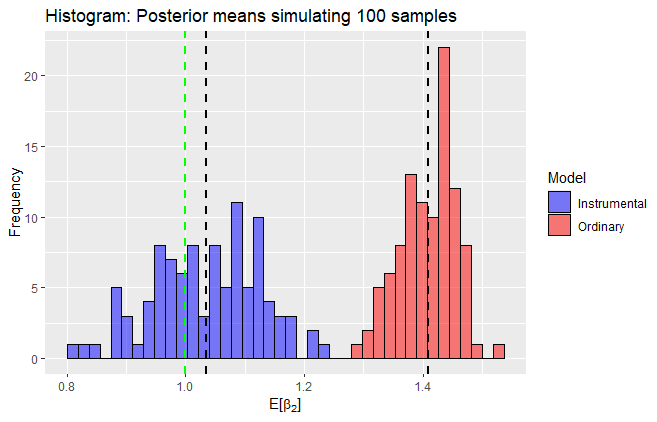
\includegraphics[width=340pt, height=200pt]{Chapters/chapter7/figures/Fig71.png}
	\caption[List of figure caption goes here]{Histogram of posterior means: Ordinary and instrumental models.}\label{fig71}
\end{figure}

Algorithm \ref{alg:IVReg} can be used to estimate the instrumental variable model using our GUI. We ask in Exercise 8 to replicate the example of the effect of institutions on per capita GDP using our GUI.  

\begin{algorithm}[h!]
	\caption{Instrumental variable model}\label{alg:IVReg}
	\begin{algorithmic}[1]  		 			
		\State Select \textit{Multivariate Models} on the top panel
		\State Select \textit{Variable instrumental (two equations)} model using the left radio button
		\State Upload the dataset selecting first if there is header in the file, and the kind of separator in the \textit{csv} file of the dataset (comma, semicolon, or tab). Then, use the \textit{Browse} button under the \textbf{Choose File} legend
		\State Select MCMC iterations, burn-in and thinning parameters using the \textit{Range sliders}
		\State Write down the formula of the structural equation in the \textbf{Main Equation} box. This formula must be written using the syntax of the \textit{formula} command of \textbf{R} software. This equation includes intercept by default, do not include it in the equation
		\State Write down the formula of the endogenous regressor in the \textbf{Instrumental Equation} box. This formula must be written using the syntax of the \textit{formula} command of \textbf{R} software. This equation includes intercept by default, do not include it in the equation
		\State Set the hyperparameters: mean vectors, covariance matrices, degrees of freedom, and the scale matrix. This step is not necessary as by default our GUI uses non-informative priors
		\State Click the \textit{Go!} button
		\State Analyze results
		\State Download posterior chains and diagnostic plots using the \textit{Download Posterior Chains} and \textit{Download Posterior Graphs} buttons
	\end{algorithmic} 
\end{algorithm}

\section{Multivariate probit model}\label{sec74}

In the multivariate probit model \cite{Edwards2003}, the response variable \( y_{il} = \{0, 1\} \) indicates that individual \( i \) makes binary choices among \( L \) mutually exclusive alternatives, where \( l = 1, 2, \dots, L \) and \( i = 1, 2, \dots, N \). Specifically, 
\begin{align*}
	y_{il} = \begin{cases}
		0, & \quad y_{il}^* \leq 0 \\
		1, & \quad y_{il}^* > 0
	\end{cases}
\end{align*}
where \( \bm{y}_i^* = \bm{X}_i \bm{\beta} + \bm{\mu}_i \sim \text{i.i.d.} \, N(\bm{0}, \bm{\Sigma}) \). Here, \( \bm{y}_i^* \) is an unobserved latent \( L \)-dimensional vector, \( \bm{X}_i = \bm{x}_i^\top \otimes \bm{I}_L \) is an \( L \times K \) design matrix of regressors, with \( K = L \times k \), where \( k \) is the number of regressors (i.e., the length of \( \bm{x}_i \)). In addition, \( \bm{\beta} = \left[\bm{\beta}_1^\top \ \bm{\beta}_2^\top \dots \bm{\beta}_k^\top\right]^\top \), where \( \bm{\beta}_j \) forms an \( L \)-dimensional vector of coefficients for \( j = 1, 2, \dots, k \).

The likelihood function for this model is given by 
\[
p(\bm{\beta}, \bm{\Sigma} \mid \bm{y}, \bm{X}) = \prod_{i=1}^N \prod_{l=1}^L p_{il}^{y_{il}},
\]
where \( p_{il} = p(y_{il}^* \geq 0) \).

Observe that $p({y}_{il}^*\geq 0)=p({\lambda}_{ll}{y}_{il}^*\geq 0)$, $\lambda_{ll}>0$. This generates identification issues because just the correlation matrix can be identified, same case as the univariate probit model where the variance of the model is fixed to 1. We follow the post processing strategy proposed by \cite{Edwards2003} to get identified parameters, that is, $\tilde{\bm{\beta}}=vec\left\{\bm{\Lambda}\bm{B}\right\}$ and the correlation matrix $\bm{R}=\bm{\Lambda}\bm{\Sigma}\bm{\Lambda}$, where $\bm{\Lambda}=diag\left\{\sigma_{ll}\right\}^{-1/2}$ and $\bm{B}=\left[\bm{\beta}_1 \ \bm{\beta}_2\dots \bm{\beta}_k\right]$.\footnote{In a Bayesian setting, a model can be non-identified; however, the posterior distribution of the model parameters exists as long as a proper prior distribution is specified \cite{Edwards2003}.}

We assume independent priors: $\bm{\beta} \sim N(\bm{\beta}_0, \bm{B}_0)$ and $\bm{\Sigma}^{-1} \sim W(\alpha_0, \bm{\Psi}_0)$. We can apply Gibbs sampling to this model, as it is a standard Bayesian linear regression model when data augmentation in $\bm{y}^*$ is used.

The posterior conditional distributions are
\begin{equation*}
	\bm{\beta}\mid \bm{\Sigma},\bm{w}\sim{N}(\bm{\beta}_n,\bm{B}_n),
\end{equation*}
\begin{equation*}
	\bm{\Sigma}^{-1}\mid \bm{\beta},\bm{w}\sim{W}(\alpha_n,\bm{\Psi}_n),
\end{equation*}
\begin{equation*}
	y_{il}^*\mid \bm{y}_{i,-l}^*,\bm{\beta},\bm{\Sigma}^{-1},\bm{y_i}\sim{T}{N}_{I_{il}}(m_{il},\tau_{ll}^2)
\end{equation*}

where $\bm{B}_n=(\bm{B}_0^{-1}+\bm{X}^{*\top}\bm{X}^*)^{-1}$, $\bm{\beta}_n=\bm{B}_n(\bm{B}_0^{-1}\bm{\beta}_0+\bm{X}^{*\top}\bm{y}^{**})$, $\bm{\Sigma}^{-1}=\bm{C}^{\top}\bm{C}$, $\bm{X}_i^{*}=\bm{C}^{\top}\bm{X}_i$, $\bm{y}_i^{**}=\bm{C}^{\top}\bm{y}_i^*$, $\alpha_n=\alpha_0+N$, $\bm{\Psi}_n=(\bm{\Psi}_0+\sum_{i=1}^N (\bm{y}_i^*-\bm{X}_i\bm{\beta})(\bm{y}_i^*-\bm{X}_i\bm{\beta})^{\top})^{-1}$,  $m_{il}=\bm{x}_{il}^{\top}\bm{\beta}+\bm{f}_l^{\top}(\bm{y}_{i,-l}^*-\bm{X}_{i,-l}\bm{\beta})$, $\bm{y}_{i,-l}^*$ is an $L-1$ dimensional vector of all components of $\bm{y}_i^*$ excluding $y_{il}^*$, $\bm{x}_{il}^{\top}$ is the $l$-th row of $\bm{X}_i$, $\bm{X}_{i,-l}$ is $\bm{X}_{i}$ after deleting the $l$-th row, $\bm{f}_l^{\top}=\bm{\omega}_{l,-l}^{\top}\bm{\Sigma}_{-l,-l}^{-1}$, $\bm{\omega}_{l,-l}^{\top}$ and $\bm{\Sigma}_{-l,-l}$ are the $l$-th row of $\bm{\Sigma}$ extracting the $l$-th element, and the sub-matrix of $\bm{\Sigma}$ extracting the $l,l$ element, and $\tau_{ll}^2=\sigma_{l,l}-\bm{\omega}_{l,-l}^{\top}\bm{\Sigma}_{-l,-l}^{-1}\bm{\omega}_{-l,l}$, and 
\begin{align*}
	\bm{X}^*=\begin{bmatrix}\bm{X}_1^*\\
		\bm{X}_2^*\\
		\vdots\\
		\bm{X}_N^*
	\end{bmatrix}, & \ I_{il}=\begin{Bmatrix} y_{il}^*> 0, & y_{il}=1\\
	y_{il}^*\leq 0 , & y_{il}=0\\
\end{Bmatrix},\text{ and}&\bm{\Sigma}=\begin{bmatrix}\bm{\omega}_1^{\top} \\ \bm{\omega}_2^{\top} \\ \vdots \\ \bm{\omega}_{L}^{\top} \end{bmatrix}.
\end{align*}

The setting in our GUI has same regressors in each binary decision. However, we can see that the multivariate probit model is similar to a SUR model in latent variables. We ask in Exercise 9 to implement a Gibbs sampling algorithm for a multivariate probit model with different regressors in each equation.\\

\textbf{Example: Self selection in hospitalization due to a subsidized health care program}

We use the dataset \textit{7HealthMed.csv}, where the dependent variable is $y = \left[\text{Hosp} \ \text{SHI}\right]^{\top}$, with $\text{Hosp} = 1$ if an individual was hospitalized in the year prior to the survey (0 otherwise), and $\text{SHI} = 1$ if the individual had subsidized health insurance (0 otherwise).

Recall that our application of binary response models aimed to uncover the determinants of hospitalization in Medellín (Colombia), where one of the regressors was a binary indicator of participation in a subsidized health care program (Section \ref{sec63}). We can use a bivariate probit model if we suspect there is dependence between the decisions regarding these two variables. A priori, we would expect that being in a subsidized health care program increases the probability of hospitalization \textit{ceteris paribus}, due to reduced costs for the patient. However, if an individual expects to be hospitalized in the future, and the factors influencing this decision are unobserved by the modeler, a feedback effect may exist from hospitalization to enrollment in the subsidized health care program.

\begin{algorithm}[h!]
	\caption{Multivariate probit model}\label{alg:MtultProbit}
	\begin{algorithmic}[1]  		 			
		\State Select \textit{Multivariate Models} on the top panel
		\State Select \textit{Multivariate Probit} model using the left radio button
		\State Upload the dataset selecting first if there is header in the file, and the kind of separator in the \textit{csv} file of the dataset (comma, semicolon, or tab). Then, use the \textit{Browse} button under the \textbf{Choose File} legend
		\State Select MCMC iterations, burn-in and thinning parameters using the \textit{Range sliders}
		\State Write down the number of cross-sectional units in the \textbf{Number of individuals: n} box
		\State Write down the number of exogenous variables in the \textbf{Number of exogenous variables: k} box
		\State Write down the number of choices in the \textbf{Number of choices: l} box
		\State Set the hyperparameters: mean vectors, covariance matrix, degrees of freedom, and the scale matrix. This step is not necessary as by default our GUI uses non-informative priors
		\State Click the \textit{Go!} button
		\State Analyze results
		\State Download posterior chains and diagnostic plots using the \textit{Download Posterior Chains} and \textit{Download Posterior Graphs} buttons
	\end{algorithmic} 
\end{algorithm}
We considered seven regressors: a constant, gender (female), age, self-perception of health status (with categories fair, good, and excellent, using bad as the reference category), and the proportion of the individual’s age spent living in their neighborhood. The last variable attempts to account for social capital, which can affect enrollment in the subsidized health insurance program, as the target population is identified by the local government \cite{Ramirez2019a}. The dataset includes 12,975 individuals who can ``choose" two options: hospitalization and enrollment in the subsidized health insurance regime.

Algorithm \ref{alg:MtultProbit} shows how to run a multivariate probit model using our GUI.
\begin{tcolorbox}[enhanced,width=4.67in,center upper,
	fontupper=\large\bfseries,drop shadow southwest,sharp corners]
	\textit{R code. Self selection in hospitalization}
	\begin{VF}
		\begin{lstlisting}[language=R]
rm(list = ls()); set.seed(010101)
Data <- read.csv("https://raw.githubusercontent.com/besmarter/BSTApp/refs/heads/master/DataApp/7HealthMed.csv", sep = ",", header = TRUE, quote = "")
attach(Data); str(Data)
p <- 2; nd <- 7; N <- length(y)/p; y <- y
Xd <- as.matrix(Data[seq(1, p*N, 2),3:9])
XcreateMP<-function(p,nxs,nind,Data){
	pandterm = function(message) {
		stop(message, call. = FALSE)
	}
	if (missing(nxs)) 
	pandterm("requires number of regressors: include intercept if required")
	if (missing(nind)) 
	pandterm("requires number of units (individuals)")
	if (missing(Data)) 
	pandterm("requires dataset")
	if (nrow(Data)!=nind*2)
	pandterm("check dataset! number of units times number alternatives should be equal to dataset rows")
	XXDat<-array(0,c(p,1+nxs,nind))
	XX<-array(0,c(p,nxs*p,nind))
	YY<-array(0,c(p,1,nind))
	is<- seq(p,nind*p,p)
	cis<- seq(nxs,nxs*p+1,nxs)
	for(i in is){
		j<-which(i==is)
		XXDat[,,j]<-as.matrix(Data[c((i-(p-1)):i),-1])
		YY[,,j]<-XXDat[,1,j]
		for(l in 1:p){
			XX[l,((cis[l]-(nxs-1)):cis[l]),j]<-XXDat[l,-1,j]
		}
	}
	return(list(y=YY,X=XX))
}
Dat <- XcreateMP(p = p, nxs = nd, nind = N, Data = Data)
y<-NULL; X<-NULL
for(i in 1:dim(Dat$y)[3]){
	y<-c(y,Dat$y[,,i])
	X<-rbind(X,Dat$X[,,i])
}
DataMP = list(p=p, y=y, X=X)
# Hyperparameters
k <- dim(X)[2]; b0 <- rep(0, k); c0 <- 1000
B0 <- c0*diag(k); B0i <- solve(B0)
a0 <- p - 1 + 3; Psi0 <- a0*diag(p)
Prior <- list(betabar = b0, A = B0i, nu = a0, V = Psi0)
# MCMC parameters
mcmc <- 20000; thin <- 5; 
Mcmc <- list(R = mcmc, keep = thin)
\end{lstlisting}
	\end{VF}
\end{tcolorbox}

\begin{tcolorbox}[enhanced,width=4.67in,center upper,
	fontupper=\large\bfseries,drop shadow southwest,sharp corners]
	\textit{R code. Self selection in hospitalization, results}
	\begin{VF}
		\begin{lstlisting}[language=R]
Results <- bayesm::rmvpGibbs(Data = DataMP, Mcmc = Mcmc, Prior = Prior)
betatilde1 <- Results$betadraw[,1:7] / sqrt(Results$sigmadraw[,1])
summary(coda::mcmc(betatilde1))
Quantiles for each variable:

				2.5%       25%       50%       75%     97.5%
var1 -1.2247602 -1.059257 -0.970870 -0.889741 -0.733411
var2  0.0269885  0.090098  0.121863  0.155585  0.220662
var3  0.0007652  0.002207  0.002925  0.003685  0.005049
var4 -0.7477149 -0.598898 -0.522549 -0.445173 -0.296718
var5 -1.4520842 -1.309922 -1.234633 -1.160468 -1.018396
var6 -1.3503717 -1.182381 -1.092511 -1.005472 -0.837939
var7 -0.1791758 -0.103506 -0.064418 -0.024499  0.051849
betatilde2 <- Results$betadraw[,8:14] / sqrt(Results$sigmadraw[,4])
summary(coda::mcmc(betatilde2))
Quantiles for each variable:
				2.5%       25%       50%       75%    97.5%
var1  0.306343  0.477265  0.564698  0.656616  0.82932
var2  0.258347  0.289819  0.305902  0.322116  0.35284
var3  0.007848  0.008656  0.009124  0.009591  0.01045
var4 -0.488810 -0.313532 -0.218459 -0.130373  0.04144
var5 -0.677686 -0.511529 -0.418139 -0.332415 -0.17322
var6 -0.703355 -0.527642 -0.433378 -0.341355 -0.16989
var7  0.164388  0.203623  0.224533  0.245306  0.28513
sigmadraw12 <-  Results$sigmadraw[,3] / (Results$sigmadraw[,1]*Results$sigmadraw[,4])^0.5
summary(coda::mcmc(sigmadraw12))
Quantiles for each variable:
2.5%       25%       50%       75%     97.5% 
-0.070515 -0.025009 -0.002895  0.018432  0.060986
\end{lstlisting}
	\end{VF}
\end{tcolorbox}

We set 20,000 MCMC iterations with a thinning parameter equal to 5. The hyperparameters are $\bm{\beta}_0 = \bm{0}_{14}$, $\bm{B}_0 = 100\bm{I}_{14}$, $\alpha_0 = 4$, and $\bm{\Psi}_0 = 4\bm{I}_2$.\footnote{Note that the order of the location coefficients in our GUI follows the equations, not the order of the regressors as in the theoretical setting presented in this section. This distinction is important for correctly setting the hyperparameters and interpreting the results of the location parameters.}

The previous \textbf{R} code demonstrates how to obtain the posterior draws using the \textit{rmvpGibbs} command from the \textit{bayesm} package. The results suggest that females, older individuals, and those who self-assess their health as poor are more likely to be hospitalized. Furthermore, females, older individuals, and those with a poor or fair self-perception of health, who have lived a larger proportion of their life in their current neighborhood, are more likely to be enrolled in the subsidized health care system. However, the results indicate that there is no unobserved correlation between the two equations, as the 95\% credible interval for the correlation is (-0.07, 0.06).

\section{Summary}\label{sec75}
In this chapter, we present the setting and posterior distributions of the most common multivariate models. The multivariate framework allows us to address \textit{endogeneity} issues by using the conditional distribution of a multivariate normal vector. Moreover, we always obtain posterior conditional distributions that belong to standard families (multivariate normal, Wishart, and truncated normal) in these models. This property enables the implementation of the Gibbs sampling algorithm for all these models.

\section{Exercises}\label{sec76}
\begin{enumerate}
	\item Show that $\mathbb{E}[u_1\text{PAER}] = \frac{\alpha_1}{1 - \beta_1\alpha_1} \sigma_1^2$, assuming that $\mathbb{E}[u_1 u_2] = 0$, where $\text{Var}(u_1) = \sigma_1^2$, in the example of the effect of institutions on per capita GDP.
	
	\item Show that $\beta_1=\pi_1/\gamma_1$, in the example of the effect of institutions on per capita GDP.
	
	\item \textbf{The effect of institutions on per capita gross domestic product continues I}
	
	Use the \textit{rmultireg} command from the \textit{bayesm} package to perform inference in the example of the effect of institutions on per capita GDP. 
	
	\item \textbf{Demand and supply simulation}
	
	Given the structural demand-supply model:
\begin{align*}
	q_i^d &= \beta_1 + \beta_2 p_i + \beta_3 y_i + \beta_4 pc_i + \beta_5 ps_i + u_{i1}, \\
	q_i^s &= \alpha_1 + \alpha_2 p_i + \alpha_3 er_i + u_{i2},
\end{align*}
where $q^d$ is demand, $q^s$ is supply, $p$, $y$, $pc$, $ps$, and $er$ are price, income, complementary price, substitute price, and exchange rate, respectively. Complementary and substitute prices refer to the prices of complementary and substitute goods for $q$. Assume that $\bm{\beta} = \left[ 5 \ -0.5 \ 0.8 \ -0.4 \ 0.7 \right]^{\top}$, $\bm{\alpha} = \left[ -2 \ 0.5 \ -0.4 \right]^{\top}$, $u_1 \sim N(0, 0.5^2)$, and $u_2 \sim N(0, 0.5^2)$. Additionally, assume that $y \sim N(10, 1)$, $pc \sim N(5, 1)$, $ps \sim N(5, 1)$, and $er \sim N(15, 1)$.

\begin{itemize}
	\item Find the \textit{reduced-form} model by using the condition that in equilibrium, demand and supply are equal, i.e., $q^d = q^s$. This condition defines the observable quantity, $q$.
	\item Simulate $p$ and $q$ from the \textit{reduced-form} equations.
	\item Perform inference for the \textit{reduced-form} model using the \textit{rmultireg} command from the \textit{bayesm} package.
	\item Use the posterior draws of the \textit{reduced-form} parameters to perform inference for the \textit{structural} parameters. Any issues? Hint: Are all \textit{structural} parameters exactly identified?
\end{itemize}

\item \textbf{Utility demand continues}

\begin{itemize}
	\item Run the \textbf{Utility demand} application using our GUI and the information in the dataset \textit{Utilities.csv}. Hint: This file should be modified to agree the structure that requires our GUI (see the dataset \textit{5Institutions.csv} in the folder \textit{DataApp} of our GitHub repository -\textbf{https://github.com/besmarter/BSTApp}- for a template).
	\item Program from scratch the Gibbs sampler algorithm in this application.   
\end{itemize}

\item \textbf{Simulation exercise of instrumental variables continues I}

\begin{itemize}
	\item Use the setting of the simulation exercise with instrumental variables to analyze the impact of a weak instrument. For instance, set $\gamma_2 = 0.2$ and compare the performance of the posterior means of the ordinary and instrumental variable models.
	\item Perform a simulation to analyze how the degree of exogeneity of the instrument affects the performance of the posterior mean in the instrumental variable model.
\end{itemize}

\item \textbf{Simulation exercise of instrumental variables continues II}

Program from scratch the Gibbs sampling algorithm of the instrumental model for the simulation exercise of the instrumental variables.

\item \textbf{The effect of institutions on per capita gross domestic product continues II}

Estimate the structural Equation \ref{eq:str1} using the instrumental variable model where the instrument of PAER is $\log(\textit{Mort})$. Compare the effect of property rights on per capita GDP of this model with the effect estimated in the example of the effect of institutions on per capita gross domestic product. Use the file \textit{6Institutions.csv} to do this exercise in our GUI, and set $\bm{B}_0=100\bm{I}_5$, $\bm{\beta}_0=\bm{0}_5$, $\bm{\gamma}_0=\bm{0}_2$, $\bm{G}_0=100\bm{I}_2$ $\alpha_0=3$ and $\bm{\Psi}_0=3\bm{I}_2$. The MCMC iterations, burn-in and thinning parameters are 50000, 1000 and 5, respectively.

\item \textbf{Multivariate probit with different regressors}

Let's do a simulation exercise where $y_{i1}^*=0.5-1.2x_{i11}+0.7x_{i12}+0.8x_{i3}+\mu_{i1}$ and $y_{i2}^*=1.5-0.8x_{i21}+0.5x_{i22}+\mu_{i2}$, $\bm{\Sigma}=\begin{bmatrix}
	1 & 0.5\\
	0.5 & 1
\end{bmatrix}$, where all regressors distribute standard normal, and $N=5000$. Use $\bm{\beta}_0=\bm{0}$, $\bm{B}_0=1000\bm{B}$, $\alpha_0=4$ and $\bm{\Psi}_0=4\bm{I}_2$. Set number of iterations 2000 and a thinning parameter equal to 5.  

\begin{itemize}
	\item Perform inference using the setting of Section \ref{sec74}, that is, assuming that $x_{i3}$ could have an effect on $y_{i2}$.
	\item Program a Gibss sampling algorithm taking into account that there are different regressors in each binary decision, that is, $x_{i3}$ does not have an effect on $y_{i2}$. 
\end{itemize}      

\end{enumerate}


